% !TeX document-id = {14b11b82-58a9-4271-b498-391391568540}
% !TeX TXS-program:compile = txs:///lualatex/[--shell-escape]

%----------------------- Преамбула -----------------------
\documentclass[ut8x, 14pt, oneside, a4paper]{extarticle}

\usepackage{extsizes} % Для добавления в параметры класса документа 14pt

% Для работы с несколькими языками и шрифтом Times New Roman по-умолчанию
\usepackage[english,russian]{babel}
\usepackage{fontspec}
\setmainfont{Times New Roman}
\usepackage[left=30mm,right=10mm,top=20mm,bottom=20mm]{geometry}
\usepackage{misccorr}
\usepackage{indentfirst}
\usepackage{enumitem}
\usepackage{pdfpages}
%\usepackage{ragged2e}
\setlength{\parindent}{1.25cm}
%\setlength{\parskip}{1em} % поменять
%\linespread{1.3}
\renewcommand{\baselinestretch}{1.5}
\setlist{nolistsep} % Отсутствие отступов между элементами \enumerate и \itemize

% Дополнительное окружения для подписей
\usepackage{array}
\newenvironment{signstabular}[1][1]{
	\renewcommand*{\arraystretch}{#1}
	\tabular
}{
	\endtabular
}

% Переопределение стандартных \section, \subsection, \subsubsection по ГОСТу;
% Переопределение их отступов до и после для 1.5 интервала во всем документе
\usepackage{titlesec}

\titleformat{\section}[block]
{\bfseries\normalsize\filcenter}{\thesection}{1em}{}

\titleformat{\subsection}[hang]
{\bfseries\normalsize}{\thesubsection}{1em}{}
\titlespacing\subsection{\parindent}{\parskip}{\parskip}

\titleformat{\subsubsection}[hang]
{\bfseries\normalsize}{\thesubsubsection}{1em}{}
\titlespacing\subsubsection{\parindent}{\parskip}{\parskip}

\newcommand{\specsection}[1]{\section*{#1}\addcontentsline{toc}{section}{#1}}

% Работа с изображениями и таблицами; переопределение названий по ГОСТу
\usepackage{caption}
\captionsetup[figure]{name={Рисунок},labelsep=endash}
\captionsetup[table]{singlelinecheck=false, labelsep=endash}

\usepackage{graphicx}
\usepackage{diagbox} % Диагональное разделение первой ячейки в таблицах

% Цвета для гиперссылок и листингов
\usepackage{color}

% Гиперссылки \toc с кликабельностью
\usepackage[linktoc=all]{hyperref}
\hypersetup{hidelinks}

% Листинги
%\setsansfont{Arial}
%\setmonofont{Courier New}

\usepackage{color} % Цвета для гиперссылок и листингов
%\definecolor{comment}{rgb}{0,0.5,0}
%\definecolor{plain}{rgb}{0.2,0.2,0.2}
%\definecolor{string}{rgb}{0.91,0.45,0.32}
%\hypersetup{citecolor=blue}
\hypersetup{citecolor=black}

\usepackage{listings}
\lstset{
	basicstyle=\footnotesize\ttfamily,
	language=XML,
	numbers=left,
	numbersep=5pt,
	tabsize=2,
	extendedchars=\true,
	breaklines=true,
	keywordstyle=\color{blue},
	frame=single,
	showspaces=false,
	showtabs=false,
	xleftmargin=17pt,
	framexleftmargin=17pt,
	framexrightmargin=-5pt,
	framexbottommargin=4pt,
	showstringspaces=false,
	inputencoding=utf8x,
	keepspaces=true
}

\usepackage{ulem} % Нормальное нижнее подчеркивание
\usepackage{hhline} % Двойная горизонтальная линия в таблицах
\usepackage[figure,table]{totalcount} % Подсчет изображений, таблиц
\usepackage{rotating} % Поворот изображения вместе с названием
\usepackage{lastpage} % Для подсчета числа страниц

\makeatletter
\renewcommand\@biblabel[1]{#1.}
\makeatother

\usepackage{color}
\usepackage[cache=false, newfloat]{minted}
\newenvironment{code}{\captionsetup{type=listing}}{}
\SetupFloatingEnvironment{listing}{name=Листинг}

\usepackage{amsmath}
\usepackage{slashbox}


\begin{document}
	
\begin{titlepage}
	\noindent\begin{minipage}{0.05\textwidth}
		
\includegraphics[scale=0.3]{inc/bmstu.png}
	\end{minipage}
	\hfill
	\begin{minipage}{0.85\textwidth}\raggedleft
		\begin{center}
			\fontsize{12pt}{0.3\baselineskip}\selectfont \textbf{Министерство науки и высшего образования Российской Федерации \\ Федеральное государственное бюджетное образовательное учреждение \\ высшего образования \\ <<Московский государственный технический университет \\ имени Н.Э. Баумана \\ (национальный исследовательский университет)>> \\ (МГТУ им. Н.Э. Баумана)}
		\end{center}
	\end{minipage}

	\begin{center}
		\fontsize{12pt}{0.1\baselineskip}\selectfont
		\noindent\makebox[\linewidth]{\rule{\textwidth}{4pt}} \makebox[\linewidth]{\rule{\textwidth}{1pt}}
	\end{center}

	\begin{flushleft}
		\fontsize{12pt}{0.8\baselineskip}\selectfont 
		
		ФАКУЛЬТЕТ \uline{<<\textbf{Информатика и системы управления}>> \hfill}

		КАФЕДРА \uline{\mbox{\hspace{4mm}} <<\textbf{Программное обеспечение ЭВМ и информационные технологии}>> \hfill}
	\end{flushleft}

	\vfill

	\begin{center}
		\fontsize{20pt}{\baselineskip}\selectfont

		\uline{\textbf{ОТЧЁТ ПО ПРОИЗВОДСТВЕННОЙ ПРАКТИКЕ}}
	\end{center}
	
	\vfill
	
	\begin{flushleft}
		\fontsize{12pt}{0.7\baselineskip}\selectfont

		Студент \uline{\mbox{\hspace{44mm}} Неумоин Дмитрий Юрьевич \hfill}
		
		Группа \uline{\mbox{\hspace{64mm}} ИУ7-63Б \hfill}
		
		Тип практики \uline{\mbox{\hspace{44mm}} Эксплуатационная \hfill}
		
		Название предприятия \uline{\mbox{\hspace{26mm}} ООО~<<ВК>> \hfill}
	\end{flushleft}	

	\vfill

	\begin{table}[h!]
		\fontsize{12pt}{0.7\baselineskip}\selectfont

		\begin{signstabular}[0.55]{p{7.25cm} >{\centering\arraybackslash}p{4cm} >{\centering\arraybackslash}p{4cm}}
		Студент & \uline{\mbox{\hspace*{4cm}}} & \uline{\hfill \textbf{Неумоин Д. Ю.} \hfill} \\
		& \scriptsize \textit{подпись, дата} & \scriptsize \textit{фамилия, и.о.}
		\end{signstabular}
	
		\vspace{\baselineskip}

		\begin{signstabular}[0.55]{p{7.25cm} >{\centering\arraybackslash}p{4cm} >{\centering\arraybackslash}p{4cm}}
			Руководитель практики & \uline{\mbox{\hspace*{4cm}}} & \uline{\hfill \textbf{Толпинская Н. Б.} \hfill} \\
			\mbox{\hspace*{1cm}} \scriptsize (от университета) & \scriptsize \textit{подпись, дата} & \scriptsize \textit{фамилия, и.о.}
		\end{signstabular}

		\vspace{\baselineskip}
		
		\begin{signstabular}[0.55]{p{7.25cm} >{\centering\arraybackslash}p{4cm} >{\centering\arraybackslash}p{4cm}}
			Руководитель практики & \uline{\mbox{\hspace*{4cm}}} & \uline{\hfill \textbf{Егоров А. С.} \hfill} \\
			\mbox{\hspace*{1cm}} \scriptsize (от предприятия) & \scriptsize \textit{подпись, дата} & \scriptsize \textit{фамилия, и.о.}
		\end{signstabular}
	
		\vspace{\baselineskip}
		
		\begin{signstabular}[0.55]{p{7.25cm} >{\centering\arraybackslash}p{4cm} >{\centering\arraybackslash}p{4cm}}
			Генеральный директор\\
			управляющей организации \\ ООО «Управляющая компания ВК» & \uline{\mbox{\hspace*{4cm}}} & \uline{\hfill \textbf{Багудина Е. Г.} \hfill} \\
			\mbox{\hspace*{1cm}} \scriptsize (от предприятия) & \scriptsize \textit{подпись, дата} & \scriptsize \textit{фамилия, и.о.}
		\end{signstabular}
	
		\vspace{\baselineskip}
		
		\begin{signstabular}[0.55]{p{7.25cm} >{\centering\arraybackslash}p{4cm} >{\centering\arraybackslash}p{4cm}}
			Оценка~~\uline{\hfill}
		\end{signstabular} 
	 
	\end{table}

	\vfill

	\begin{center}
		\normalsize \textit{\the\year~г.}
	\end{center}
\end{titlepage}
\normalsize

\pagenumbering{arabic}
\setcounter{page}{2}

\tableofcontents
\normalsize

\pagebreak

\specsection{ВВЕДЕНИЕ}

Цель производственной практики -- определить, какую часть функционала можно из баннерного демона в отдельный прокси сервер и реализовать сервис для сбора статистики сущностей <<pad>> в рекламной системе.

Задачи практики:
\begin{enumerate}
	\item провести эксперимент по вынесению части функционала из баннерного демона «bannerd» в отдельный прокси сервер, подготовить соответствующие метрики;
	\item по результатам эксперимента определить, какой функционал может быть вынесен, а какой нет;
	\item реализовать инструментарий для аналитики сущностей «pad» инвентаря площадок.
\end{enumerate}

\clearpage

\section{Характеристика предприятия}

ООО «ВК»\cite{vk} было основано в 2000 году. Основной вид деятельности --- создание и использование баз данных и информационных ресурсов. Головной офис расположен в Москве.

В проектах ВК можно общаться, играть, слушать музыку, смотреть и снимать видео, осваивать профессии и навыки, читать новости. 

Для бизнеса ВК развивает продукты и услуги для цифровизации бизнес-процессов — от интернет-продвижения до облачных сервисов.



\clearpage

\section{Описание выполнения задач}

\subsection{Экспериментальный прокси сервера}
В рамках прохождения практики бы реализован прокси сервер, стоящий перед баннерным демоном и производящий рендеринг баннера, без использования результата рендеринга. Исходный код обработчика запросов представлен в листинге \ref{code:handler}.

\begin{lstlisting}[label=code:handler, caption={Обработчик запроса прокси сервер}]
func (h ProxyTemplaterHandler) RequestHandler(ctx *fasthttp.RequestCtx) {
	// request to bannerd
	if err := h.client.Do(&ctx.Request, &ctx.Response); err != nil {
		h.logger.Error("Error in request:", log.Field("err", err))
		sentry.CaptureException(err)
		ctx.Error("Proxy host error", fasthttp.StatusInternalServerError)
		return
	}
	
	// skip result
	_, err := h.render.Render("467", render.Config{
		Db:      &store.Db{},
		Request: &ctx.Request,
	})
	
	if err != nil {
		h.logger.Error("Error in render:", log.Field("err", err))
		sentry.CaptureException(err)
		ctx.Error("Render error", fasthttp.StatusInternalServerError)
		return
	}
	
	ctx.SetStatusCode(fasthttp.StatusOK)
}
\end{lstlisting}

Разность  между средним временем ответа баннерного демона и средним времени ответа прокси сервера представлена на рисунке \ref{fig:metrics}.

\begin{figure}[hbtp]
	\centering
	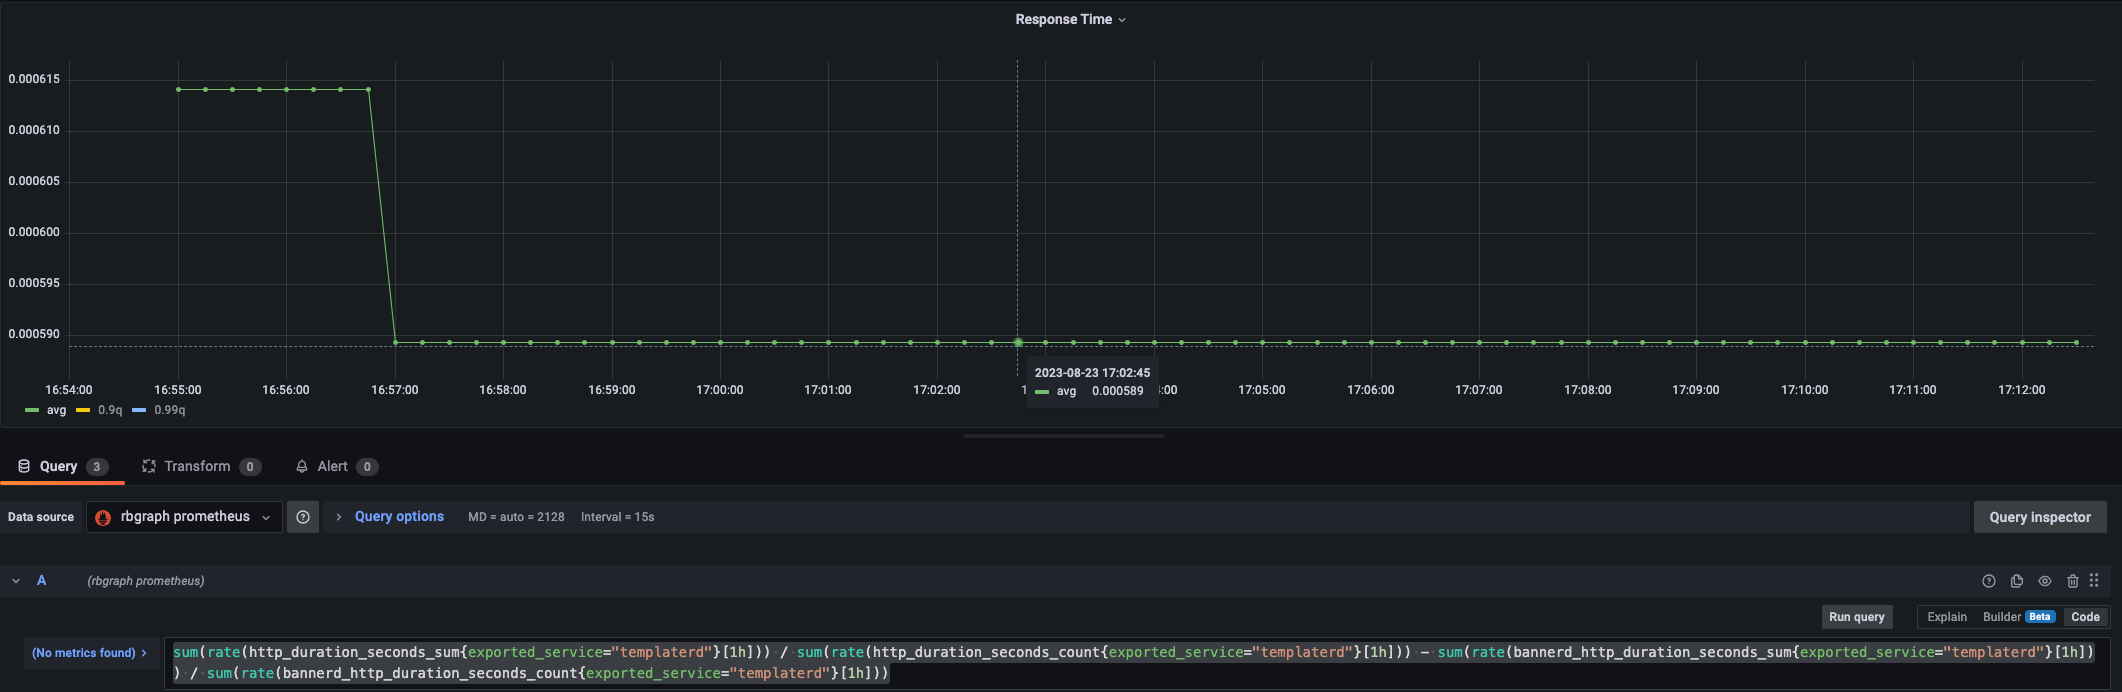
\includegraphics[width=\textwidth]{inc/metrics}
	\caption{Разность  между средним временем ответа баннерного демона и средним времени ответа прокси сервера.}
	\label{fig:metrics}
\end{figure}

\newpage

Как видно из рисунка, разность составляет порядка 500 наносекунд.  Из этого следует, что прокси сервер увеличивает время ответа на 500 наносекунд с учетом рендеринга.

\subsection{Интерпретация результатов эксперимента}

На данном этапе разработки, совместно с руководителем было принято решение, что пока можно вынести только функционал рендеринга баннера, так как вынесение большего функционала может привести к более долгим ответам сервиса, а также к многочисленным изменения кода в баннерном демоне.

\subsection{Реализация инструментария для аналитики сущностей <<pad>> инвентаря площадок}
Был разработан сервис, который раз в сутки анализирует сущности <<pad>> и распределяет их с помощью определенного алгоритма по <<слоям>> для каждого продукта. Сервис представляет возможность посмотреть слои с $gold$ по $total$, где $gold$ -- считается эталонным инвентарем, а $total$ считается фактическим, оставшиеся -- промежуточные. 

Помимо агрегатов сервис также пишем <<дельты>> в которых описано, что нужно добавить в сущность, чтобы она перешла в следующий <<слой>> . Пример таблицы агрегатов представлен на рисунке \ref{fig:agregates}.

\begin{figure}[hbtp]
	\centering
	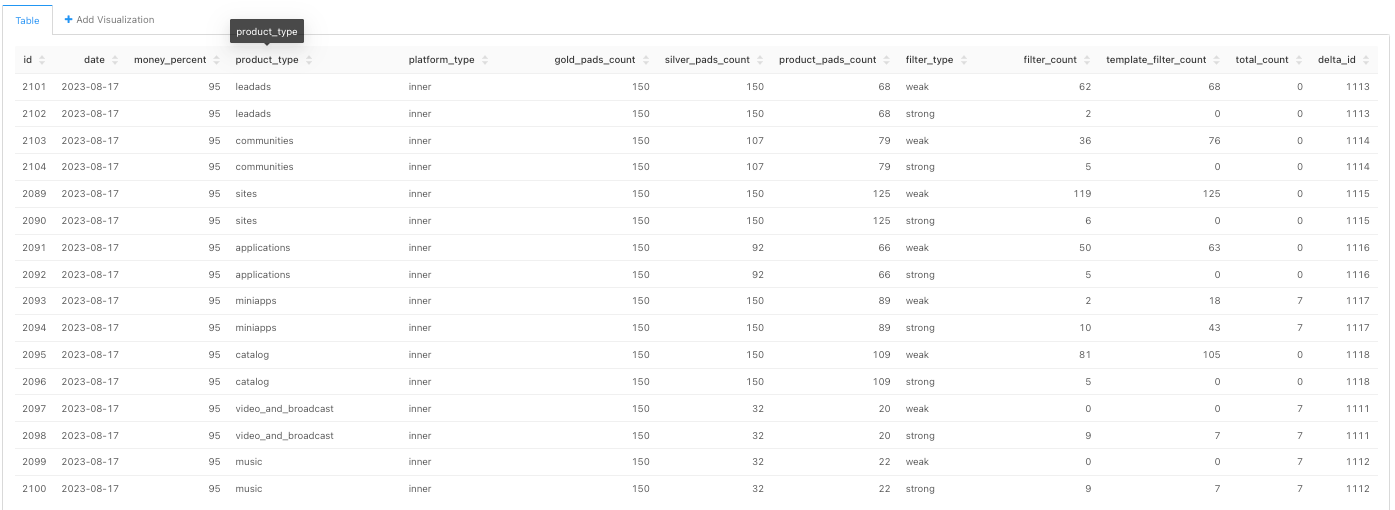
\includegraphics[width=\textwidth]{inc/agregates}
	\caption{Таблица агрегатов сущности <<pad>> по слоям.}
	\label{fig:agregates}
\end{figure}
\clearpage

\specsection{Заключение} 
В рамках производственной практики в рекламной системе ООО «ВК» была определена часть функционала для вынесения из баннерного демона в отдельный прокси сервер и реализован сервис для сбора статистики сущностей <<pad>> . Цель практики достигнута. Были выполнены следующие задачи:

\begin{enumerate}
	\item проведен эксперимент по вынесению части функционала из баннерного демона «bannerd» в отдельный прокси сервер, подготовлены соответствующие метрики;
	\item по результатам эксперимента определ  функционал для вынесения;
	\item реализован инструментарий для аналитики сущностей «pad» инвентаря площадок.
\end{enumerate}


\specsection{СПИСОК ИСПОЛЬЗОВАННЫХ ИСТОЧНИКОВ}

\begingroup
\renewcommand{\section}[2]{}
\bibliographystyle{utf8gost705u}
\bibliography{bibliography}   
\endgroup

\end{document}
